\section{Project Status}
\label{sec:project-status}

\subsection{Modeling Clock Drift}
\label{sec:modeling-clock-drift}
In previous implementations, we modeled clocks generating an event for each clock tick. Modeling drift was achieved by changing the rate of clock event generation for each node.
In the actual implementation we don't have an event for each clock tick, and drift is modeled using the Ptolemy support for multiform time. Figure \ref{fig:time} shows clock drift for one node, compared to the global model clock.

\begin{figure}
  \centering
  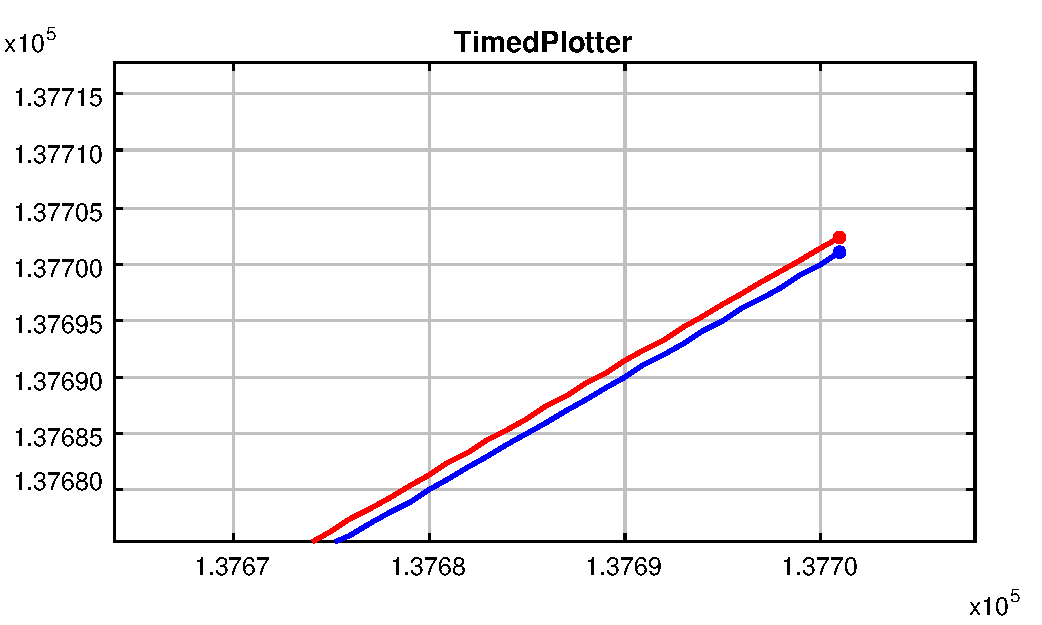
\includegraphics[width=\textwidth]{figures/time-drift.pdf}
  \caption{Clock drift modeling in Ptolemy using Multiform time}
  \label{fig:time}
\end{figure}

\subsection{Modeling the IEEE 802.15.4e state machine}
\label{sec:modeling-state-machine}

We modeled the IEEE 802.15.4e finite state machine using Ptolemy modal modes. The result is the hierarchical FSM shown in figure \ref{fig:fsm}. Figure \ref{fig:tx} shows the refinement of the \emph{transmission} state of the high level FSM. All other states of the high level FSM (\emph{reception}, \emph{SLEEP} and \emph{synchronization}) are similarly refined.

\begin{figure}
  \centering
  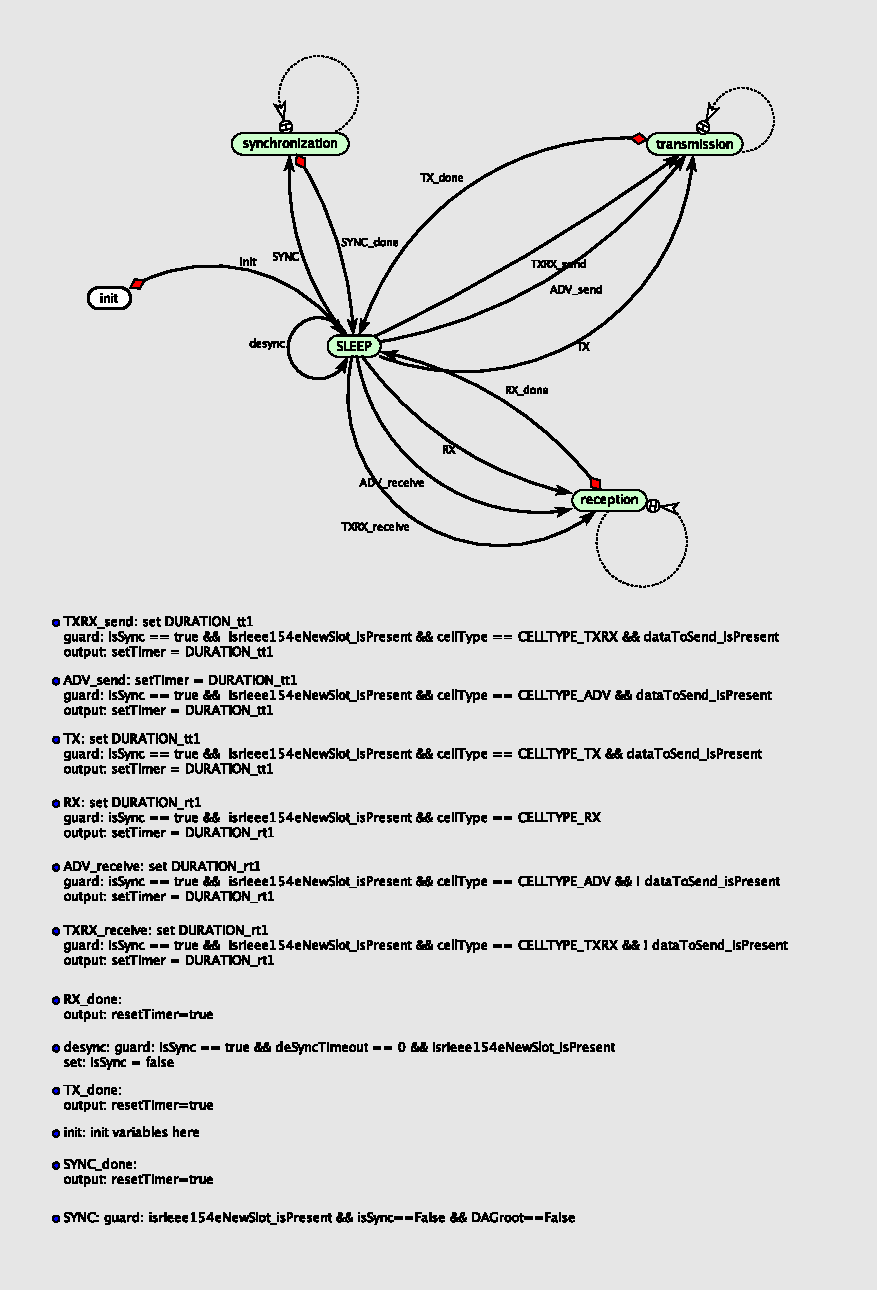
\includegraphics[width=\textwidth]{figures/FSM.pdf}
  \caption{High level FSM of the IEEE 802.15.4e protocol standard}
  \label{fig:fsm}
\end{figure}

\begin{figure}
  \centering
  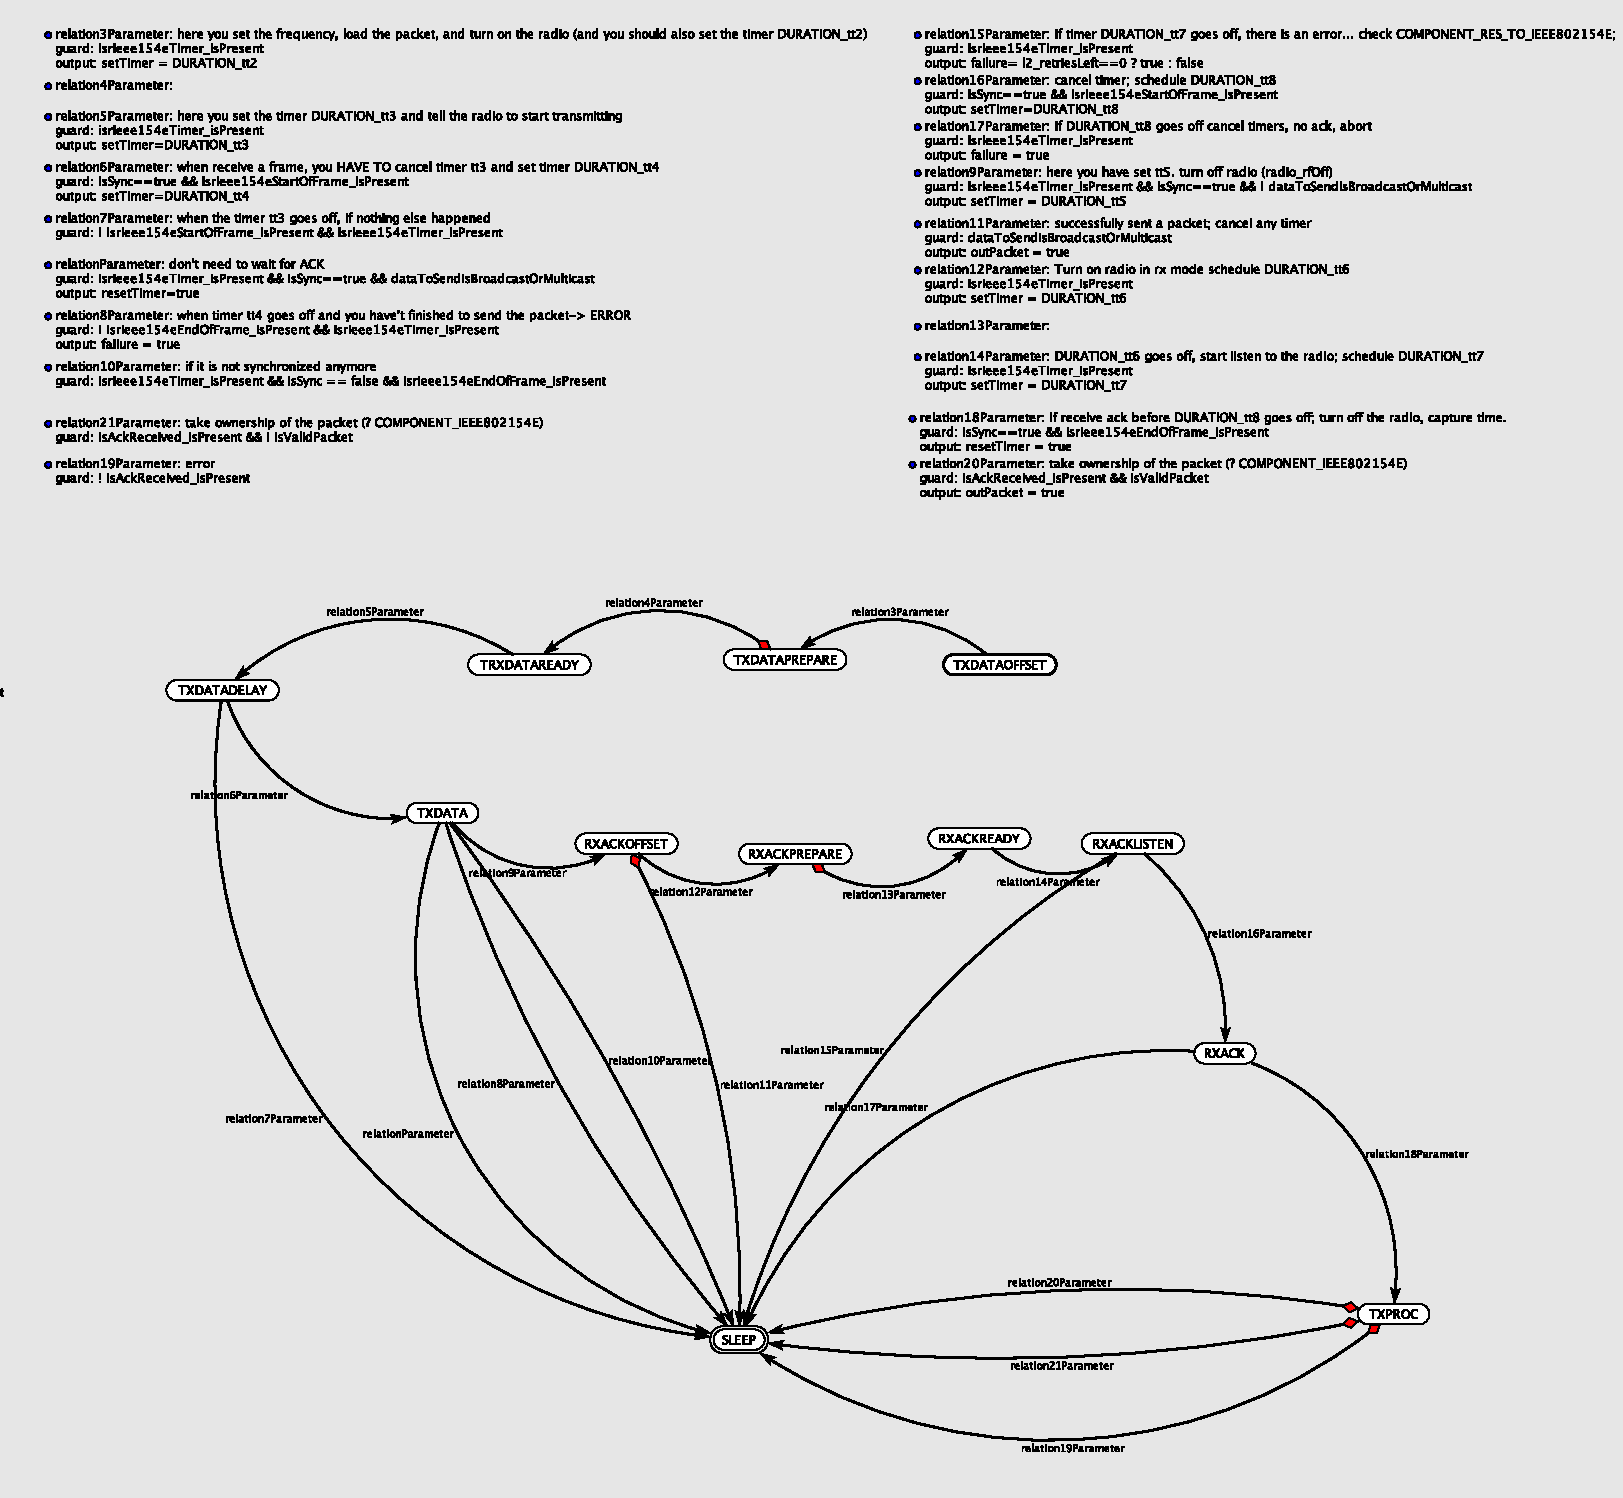
\includegraphics[width=\textwidth]{figures/TransmissionFSM.pdf}
  \caption{Transmission state refinement}
  \label{fig:tx}
\end{figure}

\subsection{Modeling the Physical Layer}
\label{sec:modeling-physical-layer}
Physical layer is modeled as a discrete event model. The physical layer is used to communicate with the MAC layer information such us the beginning and the end of the reception of a packet. Figure \ref{fig:node} shows the actual structure of a node model (a DE model), including the relation between the physical and the MAC layers.

\begin{figure}
  \centering
  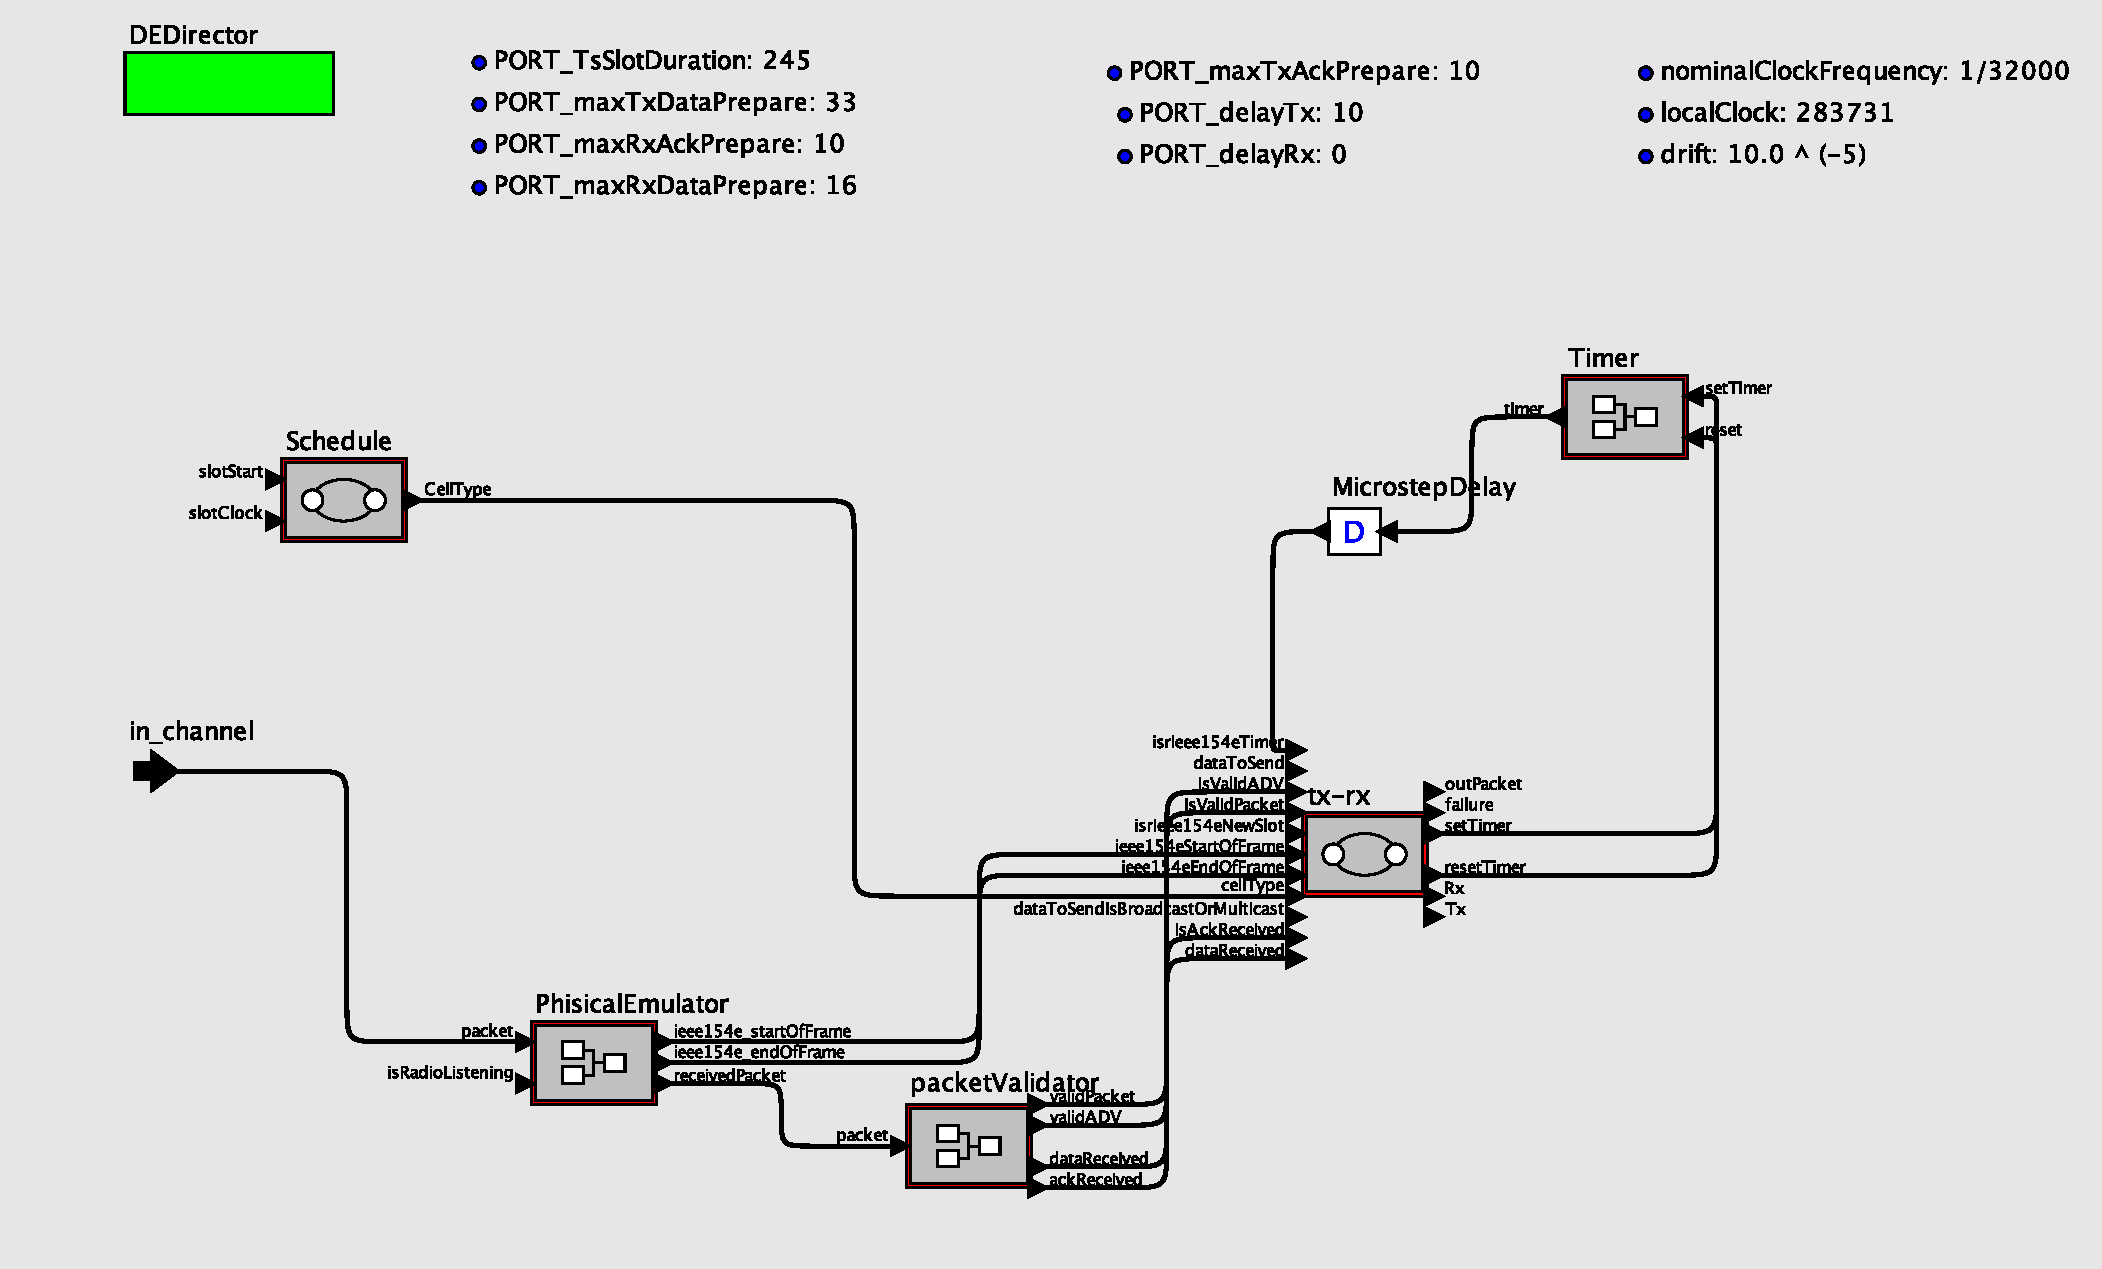
\includegraphics[width=\textwidth]{figures/WirelessNode.pdf}
  \caption{Interaction between different actors composing a node}
  \label{fig:node}
\end{figure}


\subsection{Modeling the scheduler}
\label{sec:modeling-scheduler}
In our model, the scheduler is represented as a FSM. At this point, we don't support a dynamic scheduler. In particular, our implementation of the scheduler reflects the OpenWSN implementation, where the scheduler is hard-coded in the MAC layer. Figure \ref{fig:scheduler} shows our implementation of the scheduler. Unconnected states represent other available scheduler slot types, not used in the OpenWSN implementation. Implementing a dynamic scheduler is a goal of future work.

\begin{figure}
  \centering
  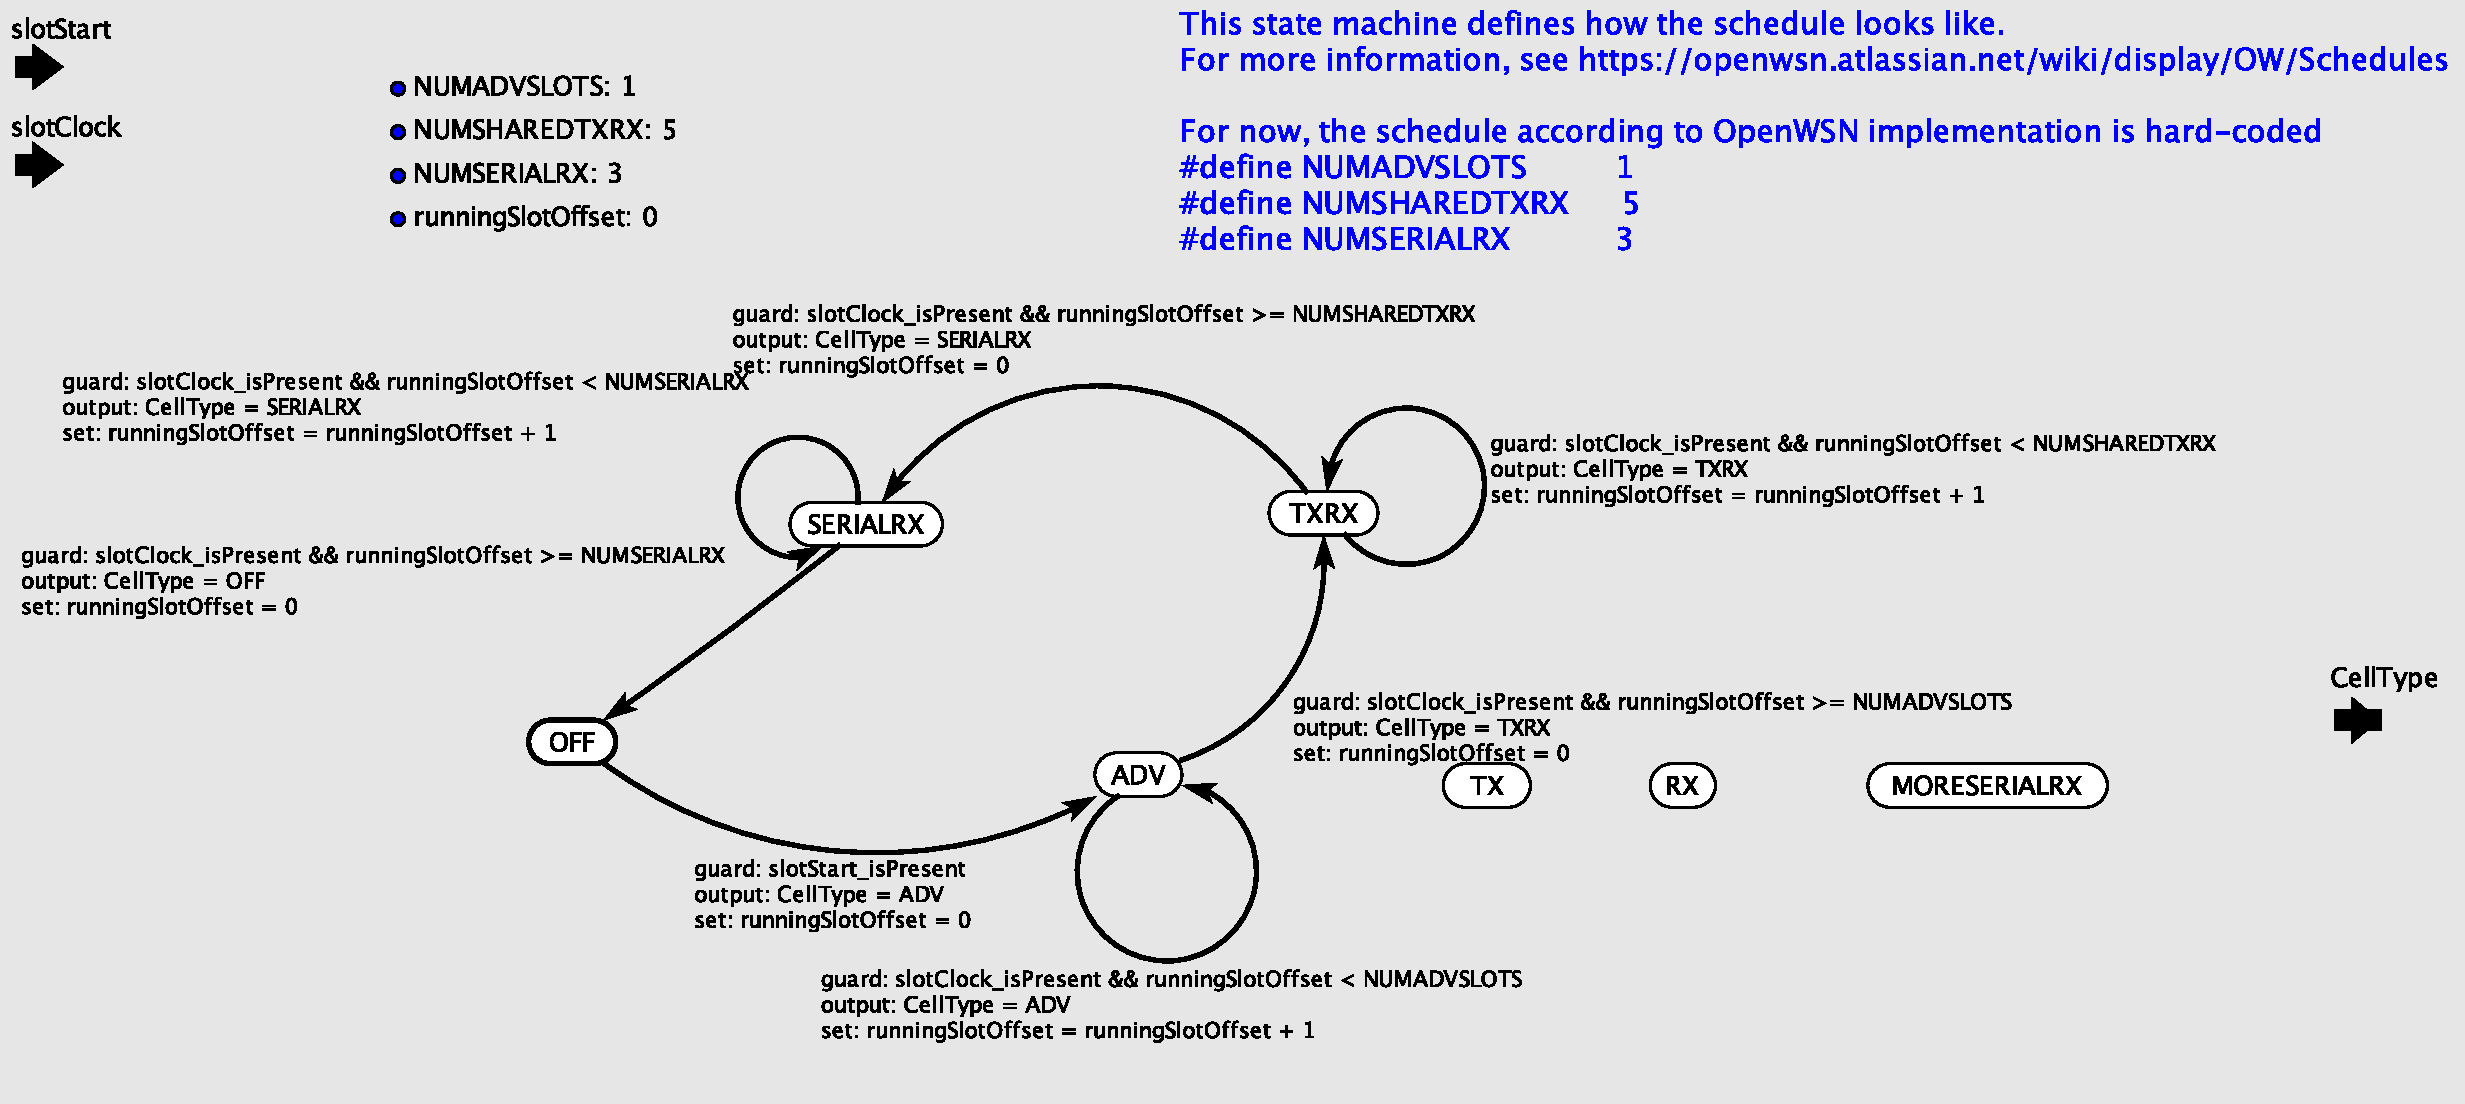
\includegraphics[width=\textwidth]{figures/Scheduler.pdf}
  \caption{Scheduler FSM}
  \label{fig:scheduler}
\end{figure}

%%% Local Variables: 
%%% mode: latex
%%% TeX-master: "report"
%%% End: 
